\chapter{Concepción y diseño de la solución}\label{chapter:solutionDesign}
En este capítulo se describe la concepción de la solución propuesta para el desarrollo 
del sistema destinado a la gestión de la información científica sobre las 
plantas medicinales cubanas, con base de conociemiento inicial en el libro de Tomás Roig. 
El capítulo está estructurado en tres secciones principales.

En primer lugar, se presenta el contexto en que se desarrolla la solución, 
explicando las motivaciones y necesidades que llevaron a su concepción. 
Posteriormente, se expone la modelación del problema, detallando cómo se definió y 
estructuró la problemática a resolver. 
Finalmente, se describe el diseño de la solución, dividida en dos subproblemas específicos, 
abordando el enfoque adoptado para dar respuesta a cada uno de ellos. 
Este análisis establece las bases conceptuales y técnicas necesarias para la 
posterior implementación y experimentación del sistema.
\newpage



\section{Contexto del problema}
La iniciativa para desarrollar el presente sistema surge a partir de un diagnóstico 
conjunto realizado entre la Universidad de La Habana y el Jardín Botánico Nacional de Cuba, 
en el contexto de un acuerdo de colaboración científica. 
Este acuerdo tiene como objetivo principal la creación de soluciones que apoyen 
la preservación, organización y difusión del conocimiento botánico en el país, 
un campo que reviste gran importancia tanto para la investigación científica, 
como para la educación y el conociemiento general de las personas.

Durante este diagnóstico, se identificó que uno de los recursos más valiosos 
en el ámbito de la botánica cubana, el libro \textit{``Plantas medicinales, aromáticas o venenosas de Cuba''} 
de Tomás Roig y Mesa, enfrentaba múltiples desafíos relacionados con su accesibilidad y 
aprovechamiento. Este libro, publicado originalmente en 1945, constituye una obra 
de referencia fundamental que recopila una vasta cantidad de información científica 
sobre la flora medicinal de Cuba, incluyendo descripciones botánicas, 
usos terapéuticos y distribución geográfica de las plantas documentadas. 
Sin embargo, a pesar de su relevancia, el acceso a esta información sigue siendo 
limitado debido a varios factores:

\begin{itemize}
    \item \textbf{Formato físico predominantemente tradicional}: Aunque existen versiones 
    digitales del libro, estas no cuentan con un diseño modular que facilite su consulta 
    o análisis de la información. Esto reduce significativamente su usabilidad en contextos 
    modernos donde predominan las herramientas tecnológicas.
    \item \textbf{Pérdida potencial del conocimiento}: El envejecimiento de los ejemplares físicos 
    y la falta de iniciativas de conservación digital de alta calidad ponen en riesgo 
    la preservación de este importante recurso.
    \item \textbf{Falta de integración en sistemas modernos de información}: Los datos 
    contenidos en el libro no están organizados de manera que puedan ser utilizados 
    en aplicaciones automatizadas, análisis de datos o sistemas de consulta avanzada.
\end{itemize}

A partir de esta realidad, el Jardín Botánico Nacional planteó la necesidad de desarrollar 
un sistema que no solo permitiera la digitalización de esta información, 
sino que también la estructurara en un formato accesible y flexible, 
capaz de responder a las demandas de diferentes tipos de usuarios. 
Este sistema debía estar alineado con el interés institucional de promover la conservación 
del patrimonio científico y natural de Cuba, a la vez que facilitara su divulgación 
a nivel nacional.

La Universidad de La Habana, como institución de referencia en la formación de 
profesionales en ciencias y tecnología, asumió el reto de apoyar esta iniciativa 
mediante el desarrollo de una solución tecnológica que integre técnicas de recuperación 
de información y bases de datos científicas. Este proyecto, en particular, 
representa un esfuerzo no solo por preservar los recursos botánicos, 
sino también por sentar las bases para la creación de sistemas similares que puedan 
aplicarse a otros ámbitos del conocimiento.





\section{Modelación del Problema}
Luego de un análisis exhaustivo de los objetivos del sistema y las necesidades 
identificadas, se han definido los siguientes requerimientos funcionales. 
Estos buscan garantizar una fiel representación de la información, así como 
lograr una interacción fluida y efectiva, 
satisfaciendo las expectativas de los distintos tipos de usuarios a los
que está destinado el producto final.

\begin{itemize}
    \item Presentar de forma estructurada y comprensible toda la información contenida 
    en las monografías del libro de Tomás Roig. Esto incluye las diferentes secciones, 
    como nombres científicos, hábitat, propiedades medicinales y composición química. 
    La representación visual debe facilitar el acceso y la interpretación de los datos, 
    con un diseño que priorice la claridad.
    \item Proveer un mecanismo avanzado de búsqueda, que permita consultar la información
    de las plantas almacenadas en el sistema, no solo mediante el nombre de las mismas, 
    sino mediante el contexto que ofrece su monografía.
    \item Incluir un módulo administrativo que permita a un usuario administrador gestionar
    la información almacenada. Esto incluye la creación de nuevas monografías de plantas, 
    la edición de información existente para corregir o actualizar datos y la eliminación 
    de registros que ya no sean relevantes o que presenten inconsistencias.
    \item Ofrecer la visualización de otras secciones relevantes del libro, que enriquezcan el
    acceso a la información.
\end{itemize}

Para comprender mejor las interacciones de los usuarios y las funcionalidades del sistema, 
se ha elaborado un diagrama de casos de uso. Este diagrama representa de manera gráfica 
las principales acciones que los diferentes tipos de usuarios pueden realizar dentro del sistema. 
Su objetivo principal es proporcionar una visión clara y estructurada de los requisitos funcionales, 
destacando los roles de los usuarios y sus respectivos casos de uso. Además, facilita la 
identificación de los límites del sistema, asegurando que las interacciones previstas cubran 
todas las necesidades y expectativas planteadas durante la modelación del problema.

En la figura \ref{fig:use-cases}, se presenta el diagrama de casos de uso correspondiente a la modelación 
propuesta del problema.

\begin{figure}[ht!]
    \centering
    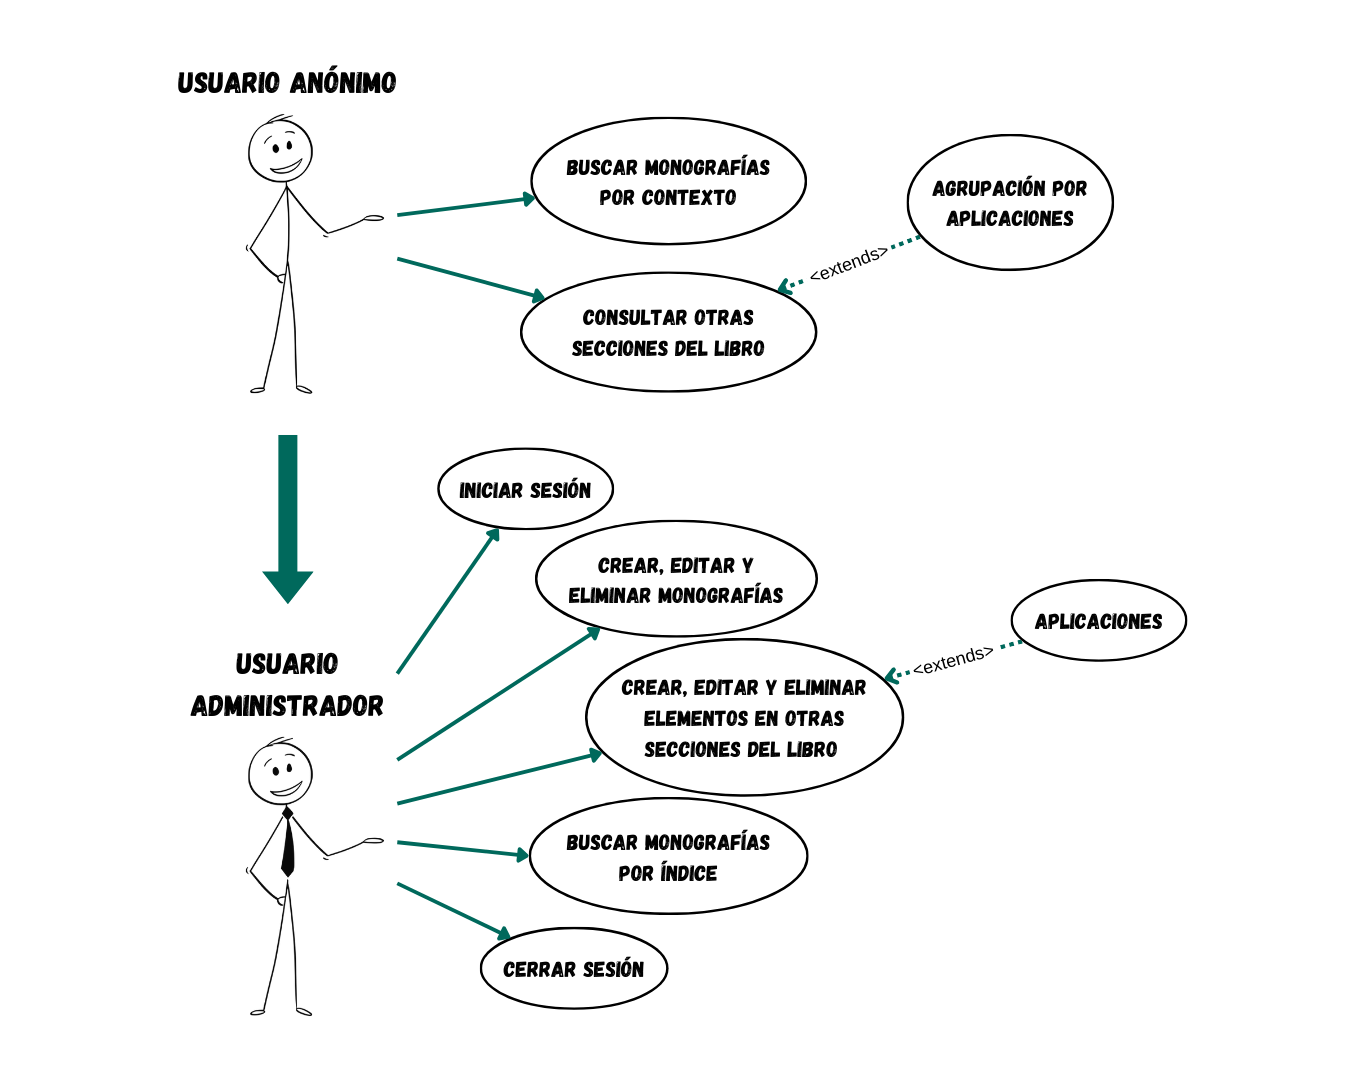
\includegraphics[width=1\textwidth]{Images/use-cases.png}
    \caption{Diagrama de casos de uso}
    \label{fig:use-cases}
\end{figure}

Es posible identificar dos subproblemas principales dentro del contexto del problema anteriormente descrito. 
Estos subproblemas están interrelacionados y son fundamentales para garantizar que el sistema cumpla 
con los objetivos establecidos:

\begin{itemize}
    \item \textbf{Problema de la extracción de la información}: Este subproblema se refiere al proceso 
    de extraer, estructurar y almacenar de manera eficiente la información contenida en el libro de Tomás Roig, 
    de forma que estos datos puedan ser consumidos por un software computacional.
    \item \textbf{Problema del sistema de gestión y visualización de la información}: Una vez 
    extraída y estructurada la información, surge el desafío de diseñar e implementar un sistema que permita 
    gestionar y visualizar eficientemente los datos.
\end{itemize}




\newpage 
\section{Diseño de la solución}
Esta sección tiene como objetivo presentar las estrategias y propuestas de diseño abstracto desarrolladas 
para abordar los subproblemas identificados en la modelación del problema. 
Estos subproblemas, centrados en la extracción de información y en la gestión y 
visualización de los datos, requieren soluciones específicas que garanticen tanto 
la fidelidad de los datos extraídos como su presentación efectiva a los usuarios finales.

En esta sección, se describirán los enfoques conceptuales diseñados para resolver cada 
uno de los subproblemas, teniendo en cuenta los requerimientos funcionales previamente establecidos. 
Se analizarán las características principales de cada solución, incluyendo sus componentes clave y cómo 
estos se integran para formar un sistema coherente y eficiente. Este análisis establecerá las bases 
para la implementación detallada del sistema.

\subsection{Extracción de la información}
\subsection{Sistema de gestión y visualización}